
\section{Challenges and Future Research}
\label{sc:challenges}
In this section, we discuss some of the unique challenges of \gls{NLC}-based RISs from both system and hardware perspectives.

%\ara{I think we are missing some system's challenges. E.g., beam switching is slower, ... }. Can we say sth about potentials btw, e.g., high-frequency design is easier?
% \subsection{Impedance matching}

% \sout{In addition to varying the propagation constant and with it the phase shift, varying the effective permittivity of a transmission line by rotating the \gls{NLC} molecules also changes its characteristic impedance. This leads to a mismatch in the lines and to a reduced bandwidth where a certain matching is achieved. 
% To improve this, wideband matching structures can be used. However, such structures achieve a wideband response by becoming electrically large and their integration into the unit cell area becomes problematic.
% In practice, resonant, frequency-selective structures are used. When designing them, at least both full-polarized states of the \gls{NLC} molecule need to be considered, $\varepsilon_{r, \parallel}$ and $\varepsilon_{r, \perp}$. This results in both i) a more complex design process, and ii) a reduced performance compared to a design optimized for a single state, since finely optimized structures for one \gls{NLC} state tend to be more frequency-selective and worsen their performance for the opposite state.}

% \sout{Along with the impedance matching due to the \gls{NLC} states, also the varying impedance on the radiating elements while scanning needs to be considered due to varying mutual coupling . Nevertheless, this is common to any antenna array and \gls{RIS}.
% Despite being very challenging, once a suitable unit cell design has been found, the single unit cell design can be repeated over the whole \gls{RIS}, so the design only needs to be optimized for a single unit cell under the assumption that it is integrated on an infinite array. When optimizing the design in a full-wave simulation software, this condition can be applied and greatly reduces the simulation time.}

% \subsection{Biasing}

% \sout{
% In the unit cell design, the integration of bias lines is not very complex. However, if each single unit cell needs to be biased, then the amount of bias lines needed linearly scales with the number of unit cells. Such bias lines are commonly realized with \gls{ITO} and can be a few \SI{}{\micro\meter} wide. For the realization of small \glspl{RIS}, the integration of electrodes going to each single cell is not problematic. However, as the size of the \gls{RIS} increases over 10×10 elements, assigning a dedicated electrode line for each unit cell becomes increasingly problematic. To solve this problem and realize large \gls{NLC} \glspl{RIS}, either i) modular approaches with multiple small \gls{RIS} \textit{tiles} or ii) active matrix type technology will have to be developed.
% Although the addition of vias as in \cite{watanabe2020ultrathin} could greatly solve the problem by routing the biasing network to a new, \gls{RF}-decoupled layer, such vias are currently not commercially available for the targeted glass substrates and thin \gls{NLC} layer thicknesses, $t_{LC}$.
% }
\subsection{Applications with slow reconfiguration}

One of the main limitations of \gls{NLC}-\glspl{RIS} is their slow response time.  There are two key factors that impact the response time: the \gls{NLC} mixture and the \gls{NLC} layer thickness, i.e., $\tau_{\rm off} \propto \gamma_{\rm rot} d_{\rm LC}^2$.
The rotational viscosity of the \gls{NLC}, $\gamma_{\rm rot}$, can be improved by using less viscous \gls{NLC} mixtures such as GT7 instead of GT5, but at the expense of increased dielectric losses. 
The \gls{NLC} thickness, $d_{\rm LC}$, strongly depends on the adopted \gls{RIS} implementation approach. 
In \glspl{RA}, \gls{NLC} thickness is commonly on the order of \SI{100}{\micro\meter} leading to a response time on the order of tens of seconds. 
Due to the resonant structure in this approach, thinner layers would lead to a significant reduction in both the bandwidth, and an increase in the insertion loss. 
On the other hand, \gls{NLC} thickness in \glspl{PA} is thin as \SI{4.6}{\micro\meter} which yields a response time in the range of tens of milliseconds (e.g., \SI{70}{\milli\second} in \cite{neuder2023compact}). 

%Note that, for example, the actual steering duration of phased arrays is about 3 times lower than the \textit{worst-case} switch-off response time. This has been verified with measured \SI{10}{\milli\second} tuning times to scan the beam from \SI{-60}{\degree} to \SI{60}{\degree} \cite{jakoby2020microwave}.

The above discussion suggests that \gls{RIS} technology should be chosen based on the applications. For scenarios where the \gls{RIS} configuration is static for an extended time period (e.g. for illumination of a blocked area), the \gls{NLC}-\glspl{RIS} with \gls{RA} implementation are suitable due to relatively lower complexity and cost. For scenarios where continuous adaptation is needed (e.g., for illuminating mobile users/devices), then \gls{NLC}-\glspl{RIS} with \gls{PA} implementation may be a preferred choice. For extremely fast reconfigurations (e.g., to track small-scale fading), other technologies such as \gls{SC}-\glspl{RIS} are needed. Although for the latter case, the overhead of channel estimation and control signaling (rather than \gls{RIS} response time) may be the bottleneck, in practice. 


%Despite the improvements in response time over the last decades, both from the material and the \gls{RF} design perspective, response times below few \SI{}{\milli\second} are currently not feasible. This indeed limits the applications for which \gls{NLC} \glspl{RIS} are suitable, and will be further discussed in Section \ref{sc:applications}.

\subsection{Undesired transient behaviour}

Due to the slow response time, the reflection pattern of \gls{NLC}-\glspl{RIS} cannot be instantaneously reconfigured, which leads to potentially undesirable transient behavior. We show this transient behavior in Fig.~\ref{fig:time response} for the following case study. It is assumed that an incident wave is normally impinged on the \gls{RIS} and then reflected first at $(\phi,\theta)=(-20,-30)$ and then at $(30,-20)$. For robustness and in order to reduce the reconfiguration overhead, wide beams of approximately 5 degrees are constructed using the quadratic phase shift design from \cite{jamali2021power}. Moreover, we show the \gls{NRCS} where the normalization is w.r.t. the maximum achievable gain by \gls{RIS} (i.e., the peak of \gls{NRCS} is 1 for speculator reflection). The transition behavior is modeled by $\tau_{\rm off}=70$~ms and $\tau_{\rm on}=10$~ms (time where $90\%$ of the phase-shift is achieved), which are taken from the \gls{PA} design in \cite{neuder2023compact}. The \gls{RIS} has a size of $50\lambda\times 50\lambda$, where $\lambda$ is the wavelength. 

Fig.~\ref{fig:time response} shows that the angular profile of \gls{NRCS} (in dB) at time instances $t=0,10,40,70,140$~ms. We can observe from this figure that the \gls{RIS} reflects the wave in many directions within the transient duration, causing interference in unwanted directions. Therefore, an interesting  direction for future research is to develop novel phase-shift configuration strategies that are aware of the \gls{RIS} transient behavior. Example problems include the design of phase-shift schemes that minimize the time to reach the desired reflection pattern or keep the interference during the transient duration below a maximum level.   

% \begin{figure*}[h]
%      \begin{subfigure}[b]{0.19\textwidth}
%          \centering
%          \includegraphics[width=\textwidth,height=3cm]{Figures/1LC transition 3D.pdf}
%      \end{subfigure}
%      %\hfill
%     \begin{subfigure}[b]{0.19\textwidth}
%          \centering
%          \includegraphics[width=\textwidth,height=3cm]{Figures/2LC transition 3D.pdf}
%      \end{subfigure}
%      %\hfill
%     \begin{subfigure}[b]{0.19\textwidth}
%          \centering
%          \includegraphics[width=\textwidth,height=3cm]{Figures/3LC transition 3D.pdf}
%      \end{subfigure}
%      %\hfill
%     \begin{subfigure}[b]{0.19\textwidth}
%          \centering
%          \includegraphics[width=\textwidth,height=3cm]{Figures/4LC transition 3D.pdf}
%      \end{subfigure}
%      %\hfill
%           \begin{subfigure}[b]{0.19\textwidth}
%          \centering
%          \includegraphics[width=\textwidth,height=3cm]{Figures/5LC transition 3D.pdf}
%      \end{subfigure}   
%     \caption{\gls{NRCS} (in dB) at several time instances when transitioning from desired reflection angles $(\phi,\theta)=(-20,-30)$ to $(30,-20)$. Cyan, white, and red rectangles are showing the current, desired, and interference directions, respectively. The \gls{RIS} response time constants are for the \gls{PA} design in \cite{neuder2023compact} and the phase-shifts are based on the quadratic phase-shift design in \cite{jamali2021power}.}
%     \label{fig:time response}
% \end{figure*}

\begin{figure*}[h]
     \begin{minipage}[t]{0.205\textwidth}
     \centering
         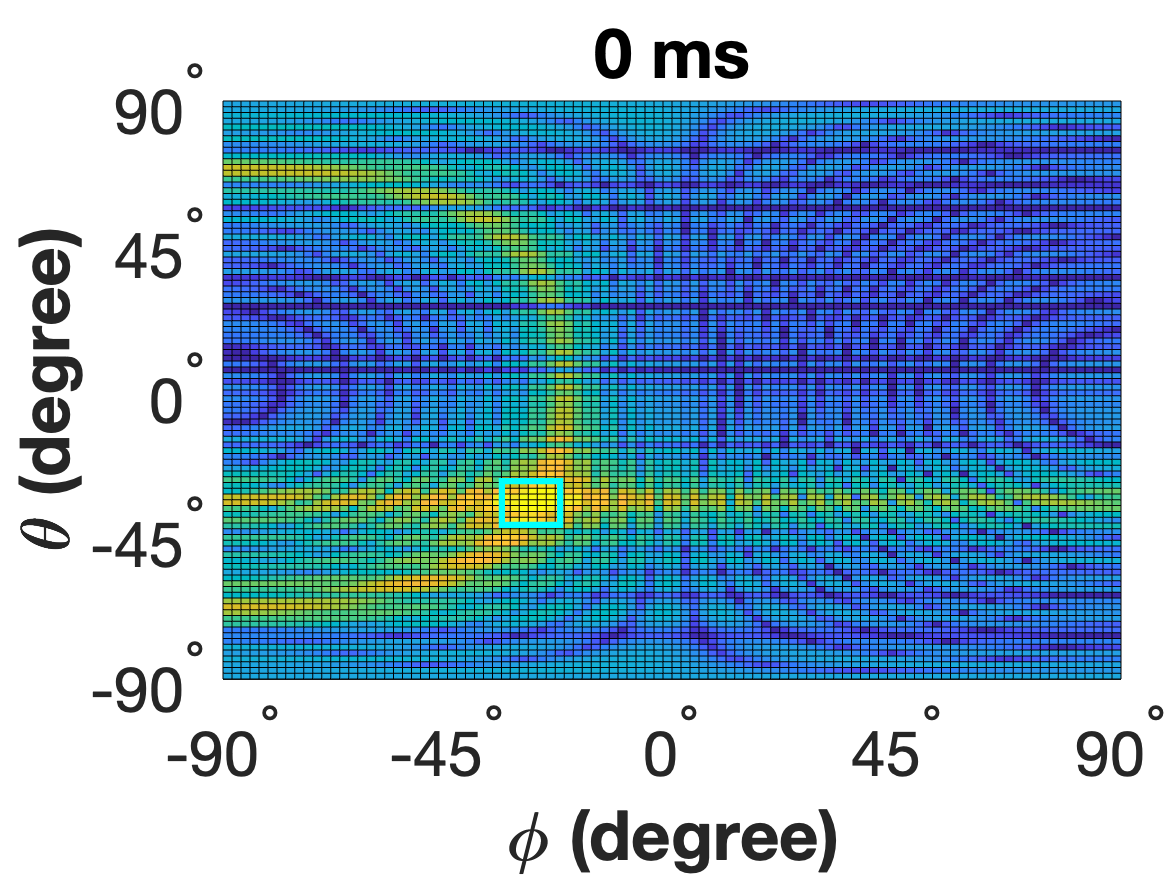
\includegraphics[width=\textwidth,height=3.5cm]{Figures/1LC_transition_3D.pdf}
   \end{minipage}
   \begin{minipage}[t]{0.19\textwidth}
     \centering
         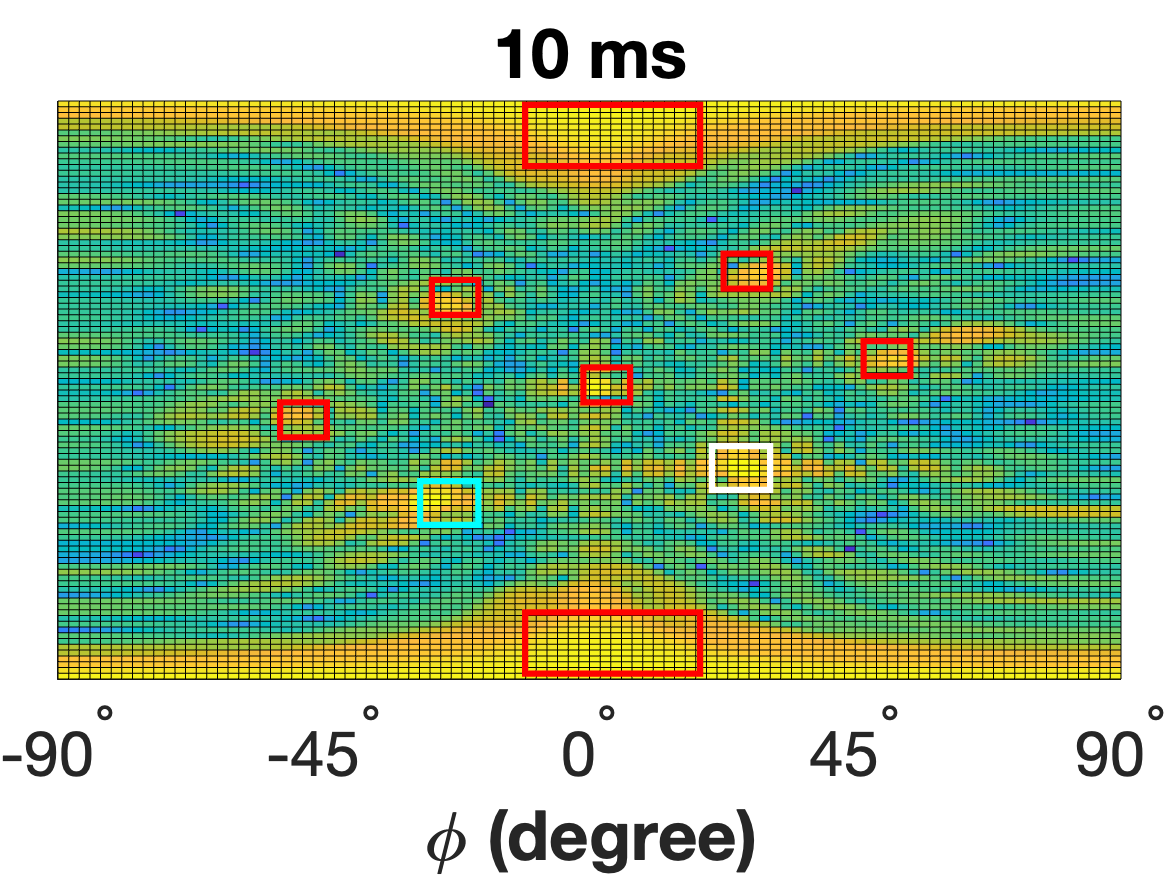
\includegraphics[width=\textwidth,height=3.5cm]{Figures/2LC_transition_3D.pdf}
   \end{minipage}
   \begin{minipage}[t]{0.19\textwidth}
     \centering
         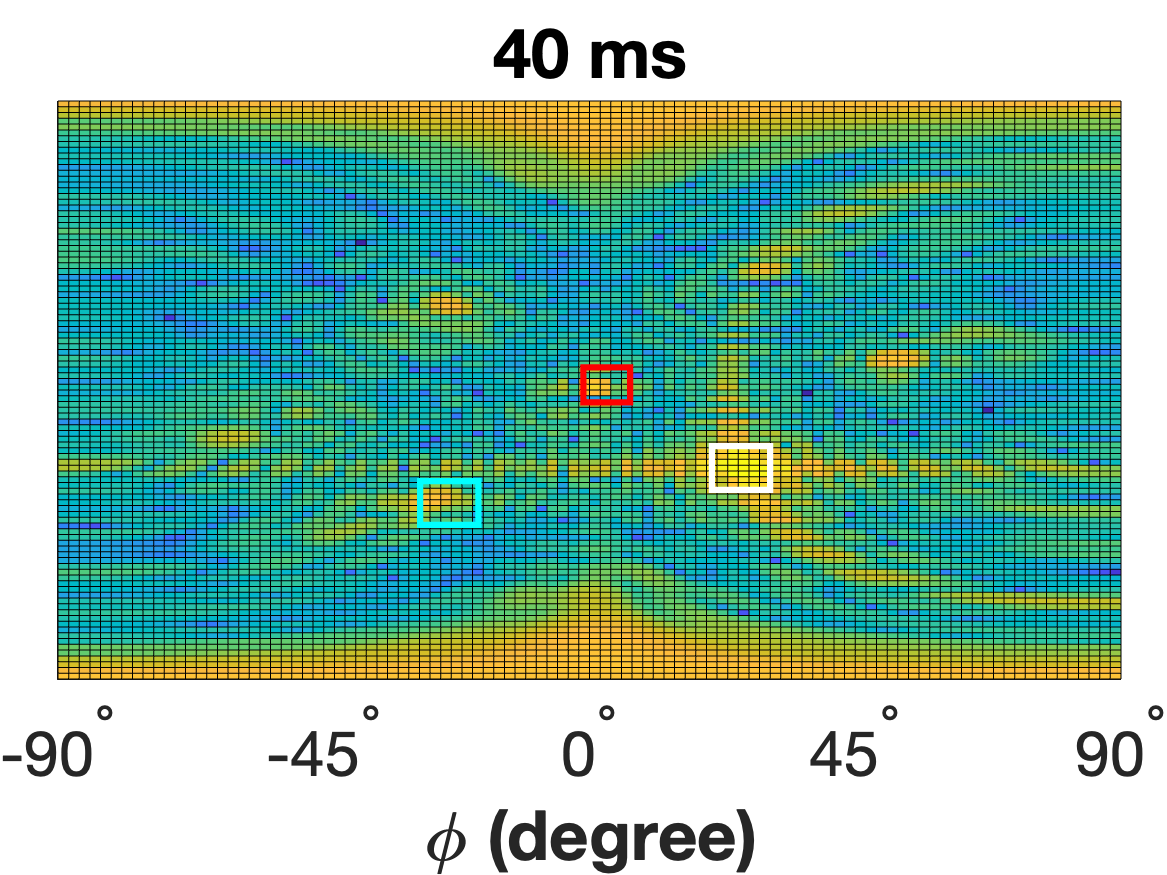
\includegraphics[width=\textwidth,height=3.5cm]{Figures/3LC_transition_3D.pdf}
   \end{minipage}
   \begin{minipage}[t]{0.19\textwidth}
     \centering
         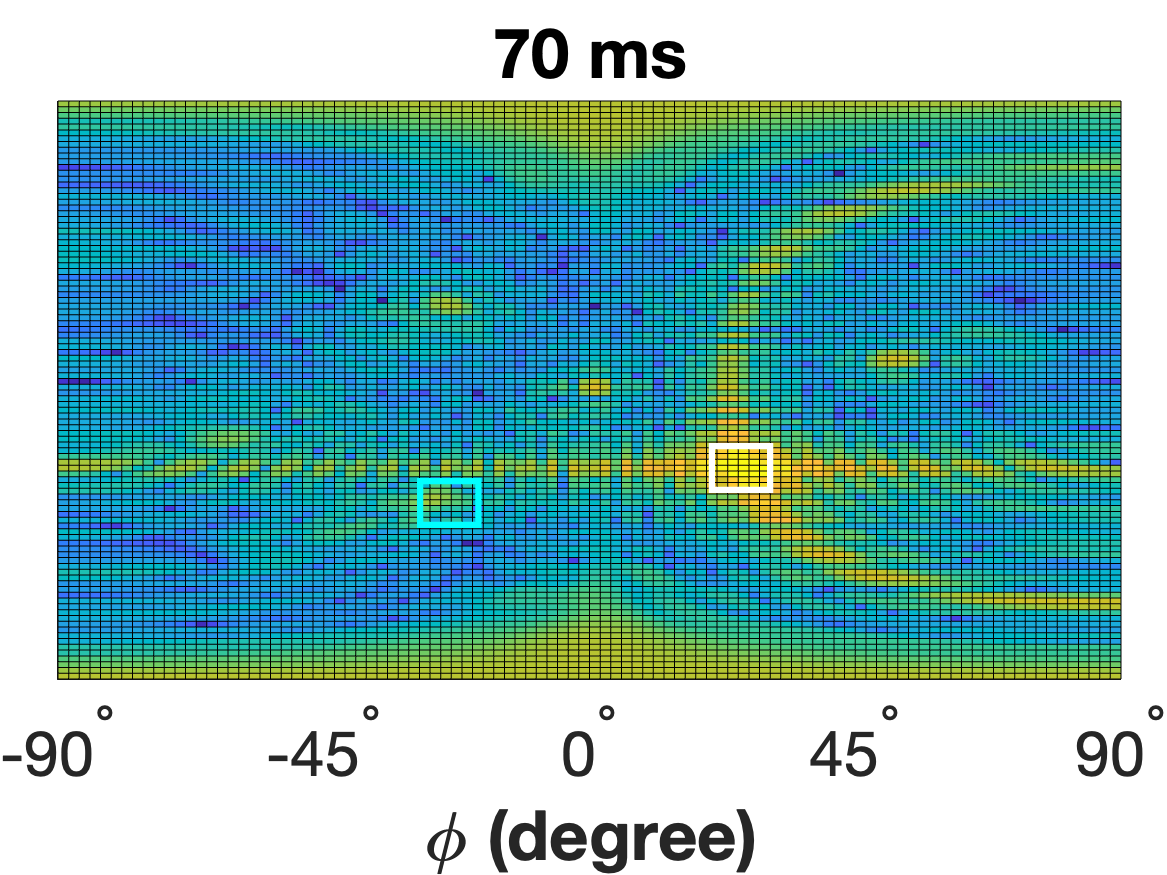
\includegraphics[width=\textwidth,height=3.5cm]{Figures/4LC_transition_3D.pdf}
   \end{minipage}
   \begin{minipage}[t]{0.205\textwidth}
     \centering
         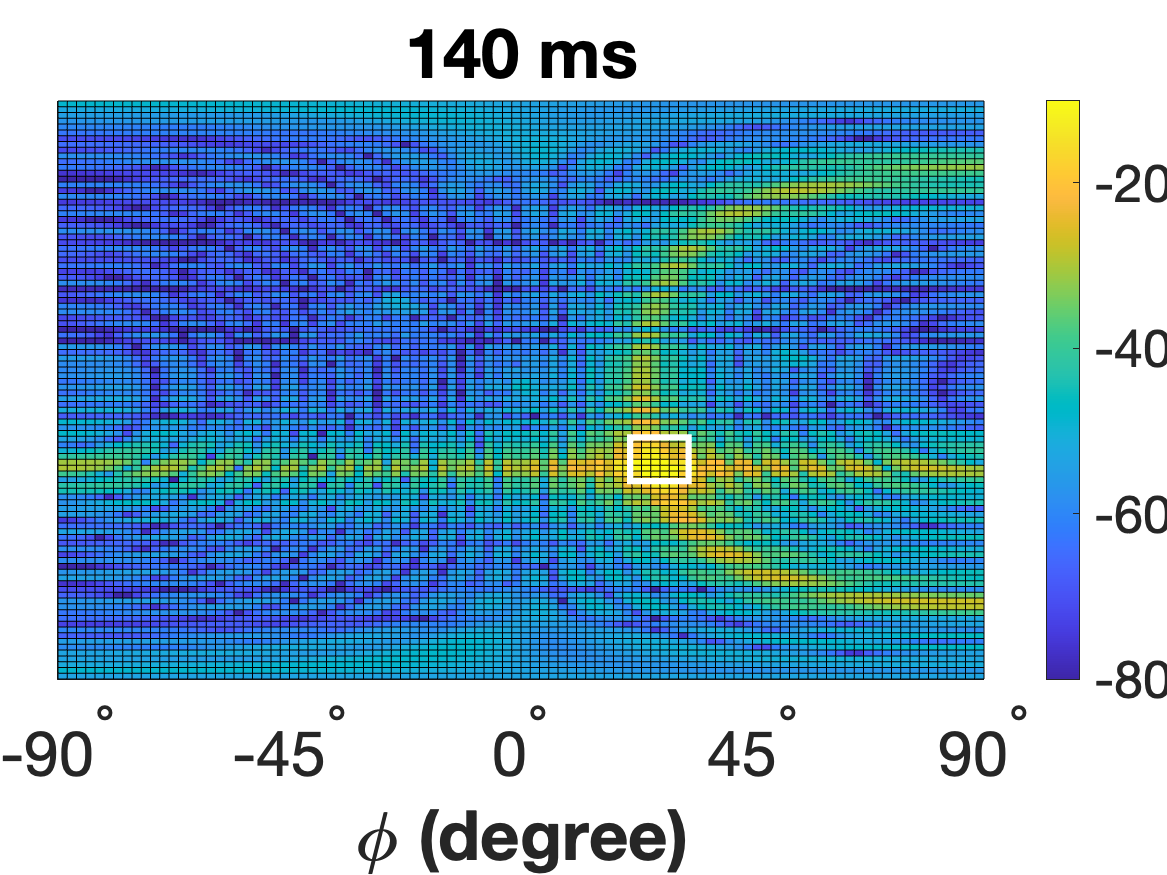
\includegraphics[width=\textwidth,height=3.5cm]{Figures/5LC_transition_3D.pdf}
   \end{minipage}
    \caption{\gls{NRCS} (in dB) at several time instances when transitioning from desired reflection angles $(\phi,\theta)=(-20,-30)$ to $(30,-20)$. Cyan, white, and red rectangles are showing the current, desired, and interference directions, respectively. The \gls{RIS} response time constants are for the \gls{PA} design in \cite{neuder2023compact} and the phase-shifts are based on the quadratic phase-shift design in \cite{jamali2021power}.}
    \label{fig:time response}
\end{figure*}

\subsection{Temperature-adaptive RIS configuration}\label{sec:temperature}
In an outdoor scenario, a \gls{RIS} needs to withstand a large range of temperatures.
For outdoor cellular systems, operation within \SIrange{-30}{+50}{\celsius} should be guaranteed. %\alejandro{does somebody know the right temperatures? It was -10 to 40, but that seems to narrow to me.}
As is illustrated in Fig.~\ref{fig:LCmolres}, the phase-shift vs. control voltage curve of the \gls{NLC}-\gls{RIS} is a function of temperature. This implies that a \gls{RIS} phase-shift configuration that is designed for temperatures in summer may not be applicable in winter. Hence, there is a need to develop temperature-aware phase-shift strategies. This requires the \gls{RIS} phase-shift behavior to be characterized offline and  the temperature to be estimated (e.g., by a thermometer deployed on the \gls{RIS}) during online operation for adapting the phase-shift design policy. Depending on the estimation error and update frequency of temperature information, robust designs that are valid for a range of temperatures may be required.


%\sout{In most cases, it can be distinguished between i) operation during the extreme temperatures, and ii) irreversible degradation of the performance after low or high temperatures have been reached. i) greatly depends on the \gls{NLC} chemical composition and can be tailored to certain applications. For example, the currently most commonly used GT7-29001 mixture has been characterized in the \SIrange{-10}{+80}{\celsius} temperature range \cite{tesmer2021temperature}. Below the minimum temperature, the material solidifies, but can be used after higher temperatures are reached again. For temperatures above \SI{999}{\celsius}, the \gls{NLC} becomes a conventional liquid and cannot be effectively tuned anymore. Furthermore, at high temperatures, a ii) progressive degradation of the organic components present in the \gls{NLC} occurs, so that the long-term performance is compromised even after cooler temperatures are reestablished.} \vahid{Such extreme temperatures is unlikely to happen in most cases. If we have space issues, we can consider removing this paragraph.}

\subsection{LC-RIS Design Tradeoffs}

In general, the maximum attainable phase-shift  of \gls{NLC} decreases with increasing temperature or decreasing frequency (see Fig.~\ref{fig:LCmolres}) \cite{tesmer2021temperature}. Therefore, to guarantee the full $360$-degree phase shift tuneability, one should design the \gls{RIS} unit cells for the maximum temperature and minimum operating frequency. This can be achieved in the \gls{PA} implementation by choosing a sufficiently large phase-shifter length $l_{\rm PS}$ (within the feasible range given the implementation constraints), since  the maximum phase-shift scales with $l_{\rm PS}$. However, as discussed in Section~\ref{Sec:Basic}, the insertion loss also scales with $l_{\rm PS}$.
Therefore, investigating the tradeoff among the maximum achievable phase shift, the resulting insertion loss, and the achievable performance (across the operating temperature and frequency) constitutes an interesting direction for future research.
To the authors' knowledge, this effect is not being considered and reported in current \gls{NLC}-\gls{RIS} designs.

%Moreover, the higher the temperature, the higher the insertion loss, and the lower the maximum attainable phase-shift  of \gls{NLC} (see Fig.~\ref{fig:LCresponse}) \cite{tesmer2021temperature}. , but this implies a larger insertion loss.
%Although the effect is very linear and not severe, it should be considered during the design of the \gls{RIS}'s phase shifters, so that 


\subsection{Biasing}
\label{ss:biasing}
For the realization of large \glspl{RIS}, the use of glass as a substrate is of great advantage due to the compatibility with current \gls{LCD} technology.
As in commercial \gls{LCD} displays, using \glspl{TFT} at each \gls{RIS} element to address them with $N+M$ (number of rows + columns) connecting lines instead of $N \times M$ (one line per element) is a meaningful approach to the challenge of biasing thousands or even millions of elements.
The additional challenge compared to common \glspl{LCD} is the higher capacitance of \gls{mm-Wave} circuits due to their larger size, requiring larger \glspl{TFT}. 
However, constraints might arise to minimize the effect of the bias lines in the \gls{RIS} operation.
This poses an additional challenge in the design of element-wise tunable \glspl{RIS} using the \gls{RA} method, since the bias lines will affect the performance of the radiating elements. 
This is commonly solved by biasing lines perpendicular to the electric-field polarization which is only possible for single, linearly polarized operation. Dual polarization designs require alternative solutions that account for the effect of the biasing lines when designing the radiating elements.
In the \gls{PA} method, this is not an issue due to the separation of the phase shifters and the radiating elements in different layers.


%\textcolor{red}{Using Indium Tin-Oxide (ITO) for the electrode feeding lines is the standard present in nearly every display due to its transparency to light.
%Nevertheless, an \glspl{RIS} does not need to be transparent to light (around 400-800 THz) but to much lower frequencies, so that novel, cheaper materials may be investigated which satisfy the requirements for low resistivity and can be cost-effectively grown (e.g., sputtered) on large surfaces.}
%\textcolor{blue}{A solution could be achieved using vias (i.e., interconnects between different layers) to bring the electrode biasing lines to an additional, RF-decoupled layer.
%Realizing through glass vias for RF circuits has been a topic of research for more than a decade, and important advances have been achieved \cite{watanabe2020ultrathin}. 
%Despite possible, the technique is not yet cost-effective for the realization of large panels.
%For this reason, the incorporation of the electrode feeding lines for the LC tuning should be achieved within the same layer as the electrodes themselves, potentially interfering with the incident, guided, and reflected electromagnetic fields.}
%\alejandro{Both colored parts could be removed to keep it short. I guess I went too much into detail.}
%\vahid{I agree that we have to make the discussion more concise. However, can we "add" a sentence about whether the biasing approach has an impact on RIS optimization? perhaps in terms of control capability?}

\subsection{Bandwidth}

\glspl{RIS} can be designed to support a single service provider (i.e., limited part of the band); an entire frequency band (e.g., 5G \SIrange{26.5}{29.5}{\giga\hertz} band), or even several bands, for example, the \SI{28}{\giga\hertz} and \SI{60}{\giga\hertz}. 
For high bandwidth systems, operating in a single band, the \gls{PA} implementation is more suitable compared to the \gls{RA}. However, \gls{RA} implementation is more suitable for multi-band operations due to the simplicity of their design. However, this comes at the cost of higher response time. Moreover, the phase-shift vs. voltage control curve of \gls{NLC}-\glspl{RIS} (see Fig.~\ref{fig:LCmolres}) changes across different frequencies within the band. Therefore, wideband phase-shift designs that exploit the frequency-dependent characteristics of the \gls{NLC}-\glspl{RIS} have to be developed.%needed in a single band, the higher the suitability of the phased array method compared to the reflectarray method. 
%In case of iii) multi-band applications, integrating multiple phase shifters in the phased array method will become an extra design effort, so the reflectarray method would be a simpler solution as long as the slower response times can be tolerable for the targeted application. Nevertheless, for wideband operations (especially scenario iii), the phase-shift vs. voltage control curve of LC-RISs (see Fig.~\ref{fig:LCresponse}) changes across different frequencies within the band. Therefore, wideband phase-shift designs that exploit the frequency-dependent characteristics of the LC-RISs have to be developed.